%!TEX root = PhD_Thesis.tex
\chapter[Human-in-the-Loop Control]{Human-in-the-Loop Control of Ultrasound-Guided Needle Steering}

\section{Introduction}
The experimental results presented in Chapter 4 showed promising accuracy in autonomous targeting of the needle tip. While these tests were performed in biological tissues, they were completed in a bench-top setting, over a relatively small needle steering workspace. Moving to a more realistic clinical environment---using a porcine cadaver in a simulated interventional radiology suite---necessitated several modifications of our bench-top techniques. The mechanical 3D ultrasound transducer used in the previous section has limited field of view relative to the size of the liver, and any motion of the transducer invalidates all existing data. (In Section~\ref{sec:AutonomousControl} the transducer was clamped relative to the tissue sample.) External tracking systems can be used to increase the ultrasound's field of view by creating panoramic data, but this necessitates additional infrastructure. The appearance of the vibrating needle in Doppler ultrasound can be highly irregular in realistic imaging arrangements. While the Doppler approach still provides an indication of needle pose, much more sophisticated segmentation algorithms, or human input, are needed for autonomous control as in Section~\ref{sec:AutonomousControl}. Finally, visualization of 3D ultrasound data, needle pose, target location, etc. requires specialized software. To allow closed-loop ultrasound-guided needle steering in a realistic clinical situation, we implemented our UKF estimation scheme using a different imaging approach. Specifically, we used freehand-3D ultrasound imaging, and manual localization of the steerable needle tip. 

This chapter is divided into three sections. Section~\ref{sec:HumanInTheLoopImplementation} describes the algorithmic, hardware, and software implementation of our clinical human-in-the-loop approach. Section~\ref{sec:HumanInTheLoopValidation} describes experimental validation of our human-in-the-loop control approach, in bench-top and simulated clinical testing. Section~\ref{sec:HumanInTheLoopResults} presents and discusses the results.

\section{Implementation}
\label{sec:HumanInTheLoopImplementation}

\subsection{Robot and Steerable Needles}
\label{sec:NS2RobotAndNeedle}
Chapter 3 presented a new articulated-tip steerable needle that showed promising curvature results in biological tissue. Unfortunately, as discussed in that chapter, the plastic construction of the miniature hinges failed too frequently to be used in a clinical setting. Chapter 6 discusses possible future improvements to the hinge design. In this chapter, we applied the exaggerated tip geometry suggested by the results of Chapter 3, but used a flexure tip, consisting of a rectangular Nitinol wire plastically deformed to the desired tip angle. This tip is able to pass through an introducer sheath because of the large elastic range of Nitinol, but still returns to its bent shape inside tissue. A similar flexure tip was previously proposed by Swaney et al.~\cite{Swaney2013}. Fig.~\ref{fig:NS2AndNeedle} shows the flexure tip steerable needle and the robot used to drive it in this chapter.

\begin{figure}[!ht]
\centering
\includegraphics[width = \columnwidth]{./Images/Chapter5/NS2RobotAndNeedle/NS2RobotAndNeedle.jpg}%
\caption[Robot and flexure-tip steerable needles]{Portable needle steering robot with positioning arm and handle, flexure-tip steerable with integrated anti-buckling sheath and luer connector fitting for introducer needle.}
\label{fig:NS2AndNeedle}
\end{figure}  

\subsection{Control Modes}
Our implementation of human-in-the-loop control allows the user to select between joint-space control of the needle steering robot and task-space control of the needle tip position. In joint-space control, the user uses a 3D mouse (SpaceNavigator; 3Dconnexion, Boston, MA) to directly control the insertion and rotation of the needle steering robot's two DOF. Using a rate-control scheme, uniaxial displacement of the 3D mouse is mapped to insertion velocity, while uniaxial rotation of the 3D mouse is mapped to rotation speed. The remaining inputs of the 3D mouse are not used. Fig.~\ref{fig:InputDevices} shows the 3D mouse.

\begin{figure}[!t]
\centering
\includegraphics[width = \columnwidth]{./Images/Chapter5/InputDevices/InputDevices.pdf}%
\caption[Input devices for robot control]{Input devices for human-in-the-loop control of robotic needle steer: (a) A tablet is used to select targets and measure the needle tip position in the stream of 2D ultrasound images. (b) A 3D mouse is used for rate control of the steerable needle insertion and rotation.}
\label{fig:InputDevices}
\end{figure}  

In task-space control, the user selects target positions directly in the live 2D ultrasound image using a tablet interface (Cintiq 13; Wacom Co., Vancouver, WA). The tablet interface is shown in Fig.~\ref{fig:InputDevices}. The robot then steers the needle towards the target semi-autonomously, with feedback based on the output from the UKF estimation scheme described in Chapter 4. The estimator is updated without measurement feedback (i.e., based on the process model) at the ultrasound machine's native framerate. After every 10~mm of insertion, the system requires a tip position measurement, which the user provides by scanning over the needle tip and localizing it using the tablet interface. The estimation scheme is implemented exactly as described in Chapter 4 with two exceptions. First, the process and measurement noise levels were again experimentally characterized for the flexure needle and manual measurements, and the filter gains were adjusted accordingly. Second, the manual measurements only provided feedback on tip position, so tip orientation feedback was taken directly from the output of the estimator, with extremely low gain (high variance). This approach avoided practical computational problems related to matrix inversion and manipulation. 

Based on the output of the UKF estimation scheme, the needle was controlled using a sliding mode control, as described by Rucker et al.~\cite{Rucker2013}. In this control scheme, needle tip rotation is constantly adjusted so that the direction of needle curvature points towards the target. This approach eliminates the need for explicit duty-cycle control. 

\begin{figure}[!t]
\centering
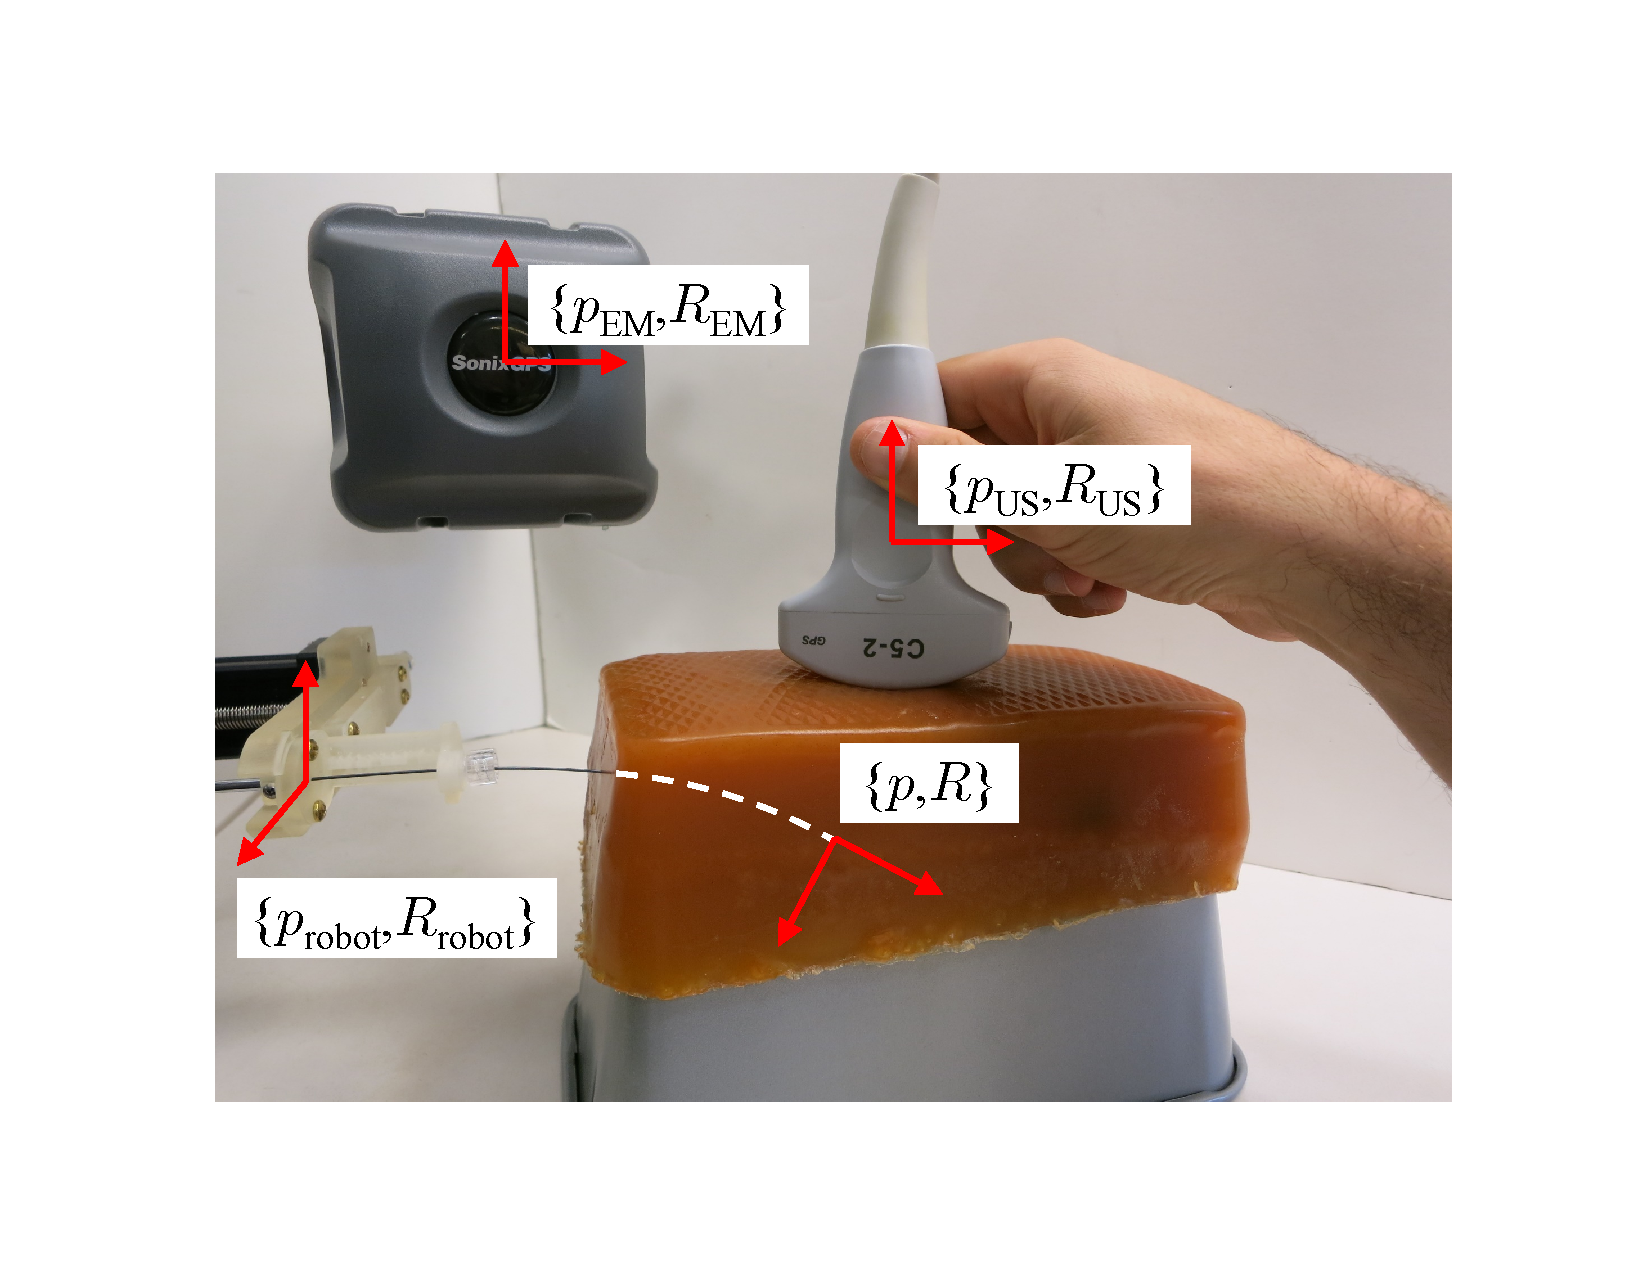
\includegraphics[width = \columnwidth]{./Images/Chapter5/Freehand3DUS/Freehand3DUS.pdf}%
\caption[Freehand 3D ultrasound imaging arrangement]{Freehand 3D ultrasound imaging arrangement and relevant coordinate systems. The pose of the needle tip, defined by $\{p,R\}$, is measured using a 2D ultrasound transducer with integrated tracking element and pose defined by $\{p_{\text{US}},R_{\text{US}}\}$. The transducer is tracked relative to electromagnetic base station with pose $\{p_{\text{EM}},R_{\text{EM}}\}$. The tracker information is referred to the robot frame $\{p_{\text{robot}},R_{\text{robot}}\}$ using a tracking element in the distal section of the robot, and a stylus calibration.}
\label{fig:freehand3DUS}
\end{figure}  

\subsection{Freehand 3D Doppler Ultrasound Imaging}
As in the previous chapters, a SonixMDP ultrasound console (Ultrasonix Medical Corp., Richmond, Canada) was used for imaging. Unlike in the previous chapters, a 2D curvilinear transducer (C5-2/60) with an integrated electromagnetic tracking element was used. Fig.~\ref{fig:freehand3DUS} depicts this arrangement. The calibrated electromagnetic tracking system, branded as SonixGPS by Ultrasonix, allows the 3D context of the 2D ultrasound image data to be resolved in real time. 

As in Chapter 2, external vibrations were applied to the proximal end of the steerable needle shaft. However, in this chapter, a spring-loaded clip was used to attach a vibration motor (a miniature DC motor spinning a small eccentric mass) to the steerable needle shaft. Fig.~\ref{fig:Buzzer} shows the new vibration device. Compared to the integrated piezoelectric buzzer described in Chapter 2, this system has the advantages that is completely disposable if contaminated with bodily fluids, and it can be visually monitored during insertion and retraction to ensure good coupling. These characteristics were identified as necessary after early clinical testing.

\begin{figure}[!t]
\centering
\includegraphics[width = 0.8\columnwidth]{./Images/Chapter5/Buzzer/Buzzer.jpg}%
\caption[Disposable buzzer]{Disposable buzzer for ultrasound Doppler imaging. A 3D-printed spring-loaded clip attaches a vibration motor to the steerable needle shaft. The unit is battery powered and entirely disposable. Motion along the needle shaft is constrained by an enclosure.}
\label{fig:Buzzer}
\end{figure}  

\subsection{Visualization and Control Software}
A custom graphical user interface (GUI) was developed using Qt, for human-in-the-loop control. The GUI is shown in Fig.~\ref{fig:GUI}. The clinician user views both a live 2D ultrasound image streamed from the SonixMDP console, as well as a live 3D visualization of the robot pose, transducer pose, estimate, and target, as defined using the SonixGPS tracker. The GUI is optimized for a tablet interface. Controls allow the user to select between the two control modes (joint-space control and task-space control). The user can use the tablet interface to set a the target point by clicking in the live 2D ultrasound image. Measurements of the steerable needle tip's position are similarly performed by clicking in the live 2D ultrasound image. 

\begin{figure}[!t]
\centering
\includegraphics[width = 0.9\columnwidth]{./Images/Chapter5/GUI/GUI.jpg}%
\caption[Software interface]{Software interface for human-in-the-loop control. A screenshot shows the software during initial insertion of the robot, while the steerable needle tip is still within the introducer needle. Three panels are shown: (left) the live 2D ultrasound image with the current tip frame estimate over the hyperechoic needle shaft, (top right) the 3D visualization showing the ultrasound transducer pose, robot pose, tip frame estimate, and target (blue sphere), (bottom right) software control buttons and robot status readout.}
\label{fig:GUI}
\end{figure}  

%------------------------------------------------------------------------------------------
%------------------------------------------------------------------------------------------
\section{Experimental Validation}
\label{sec:HumanInTheLoopValidation}
%------------------------------------------------------------------------------------------
%------------------------------------------------------------------------------------------
\subsection{Quantification of Process and Measurement Noise}
As in Chapter 4, we first quantified process noise and measurement noise using our new robot and imaging arrangement. Process noise was again quantified by using a magnetic tracking system to precisely measure the motion of a steerable needle tip during incremental insertion along constant curvature paths. In this testing, a flexure-tip steerable needle with $l = 10$~mm and $\alpha = 45$~degrees was used. The needle was inserted along a minimum-radius-of-curvature path at a constant insertion velocity of XX mm/s, and no rotation. The pose of the needle tip after each incremental step was compared with what was expected based on the previous pose and the process model. Although the insertion increment varied slightly due to software timing, it was generally about 0.2~mm. The needle was inserted along six paths, with 617 total measurements captured. The initial tip frame orientation was defined in the robot frame based on fixture geometry and the initial joint values $\theta$ and $\l$. Radius of curvature $\rho$ for the needle was also measured using the magnetic tracking data and the least-squares fitting approach described in Chapter~3. Data analysis was performed offline using Matlab. 

Measurement noise was quantified by comparing manual tip localization results from repeated freehand-3D ultrasound scans of steerable needles in porcine liver tissue. Five repeated measurements were performed at each tip position, with 200 total measurements over five needle insertions. For each measurement, the user scanned over the needle with the ultrasound transducer, and manually selected the location of the steerable needle tip using the tablet and stylus. Data analysis was again performed offline in Matlab.

\subsection{Accuracy of Estimation Scheme}
We quantified the accuracy of our UKF estimation scheme in this application by comparison with the electromagnetic tracking system over a series of steering trials. Over four insertions in \textit{ex vivo} porcine liver, the needle was steered while alternating between joint-space and task-space control. On each control update (synchronized to the ultrasound framerate), the calibrated electromagnetic tracker reading and UKF estimate were saved. Comparison was performed offline in Matlab.

\subsection{Clinical Needle Steering Experiments}
Fig.~\ref{fig:CadaverSetup} shows the experimental setup for the clinical needle steering experiments. A fresh pig carcass with an undisturbed liver was obtained for testing. To prevent coagulation and preserve the mechanical properties of the liver as much as possible, heparin was administered at a dosage of 300 IU/kg prior to euthanasia. The carcass was placed in supine position on a standard interventional radiology suite table, and was restrained to prevent tissue motion. 

\begin{figure}[!t]
\centering
\includegraphics[width = \columnwidth]{./Images/Chapter5/CadaverSetup/CadaverSetup.jpg}%
\caption[Experimental setup for clinical needle steering]{Experimental setup. The pig carcass is mounted in supine position on the table. The needle steering robot is secured to the table rails, and connected to an introducer sheath to allow access to the liver through skin and subcutaneous fat. A second introducer sheath allows placement of target coils.}
\label{fig:CadaverSetup}
\end{figure}  

After exploratory ultrasound imaging, multi-loop-coil fiducials were implanted in the liver to serve as targets. These fiducials are designed to be visible in CT imaging, but can also be visualized in ultrasound because of the gas trapped in the coils. A 15-gauge introducer needle was used to place each fiducial, and the needle was left in place during steering to aid in target identification. The three targets were increasingly difficult based on the curvature and insertion distance required to reach them from the introducer. Target 1 was located fairly close to the introducer, but required steering to avoid a section of portal vein. Target 2 was posterior to the gallbladder, and was placed by puncturing the gallbladder sack. Target 3 was also posterior to the gallbladder, but required the steerable needle to curve around the posterior aspect of the gallbladder. Fig.~\ref{fig:CadaverTargetsUS} shows the approximate locations of the three targets, projected onto the ultrasound image plane.

\begin{figure}[!t]
\centering
\includegraphics[width = \columnwidth]{./Images/Chapter5/CadaverTargetsUS/CadaverTargetsUS.pdf}%
\caption[Entry vector, targets and obstacles in cadaver liver]{Entry vector, targets and obstacles in cadaver liver. Three fiducials (numbered) were implanted around the gallbladder to provide targets for closed-loop needle steering. The targets were not all located within the imaging plane, and locations are approximate. The introducer needle and approximate initial path of the steerable needle are indicated, as are the gallbladder and liver boundary. }
\label{fig:CadaverTargetsUS}
\end{figure} 

After implantation, the target was localized in ultrasound using the interface software, and the needle steering robot was used to place the tip of the steerable needle at the target fiducial using human-in-the-loop control. The steerable needle accessed the liver in an anterior subcostal approach, through a 15-gauge, XX-cm-long introducer needle. Steering proceeded in 10-mm increments, with a manual needle tip localization required after each increment. The needle was localized using a combination of B-mode and power Doppler ultrasound; users would alternate between the modes and activate the vibration device as needed depending on needle visibility. Typically, one user manipulated the ultrasound transducer, while a second localized the target and steerable needle in the ultrasound images. Fig.~\ref{fig:CadaverUsers} shows these interactions. In this testing, a standard mouse and monitor was used in place of the tablet interface to allow the entire team to view the images. In the future, one user could perform both the imaging and localization using the described tablet interface. Once the steerable needle reached the target depth, as measured by the output of the needle estimator, needle insertion stopped. A DynaCT scan was then captured using an Artis zeego imaging system (Siemens Medical Solutions, Inc.; Malvern, PA). Accuracy of tip placement was determined by measuring the distance between the tip of the steerable needle and the target fiducial in the DynaCT data.

\begin{figure}[!t]
\centering
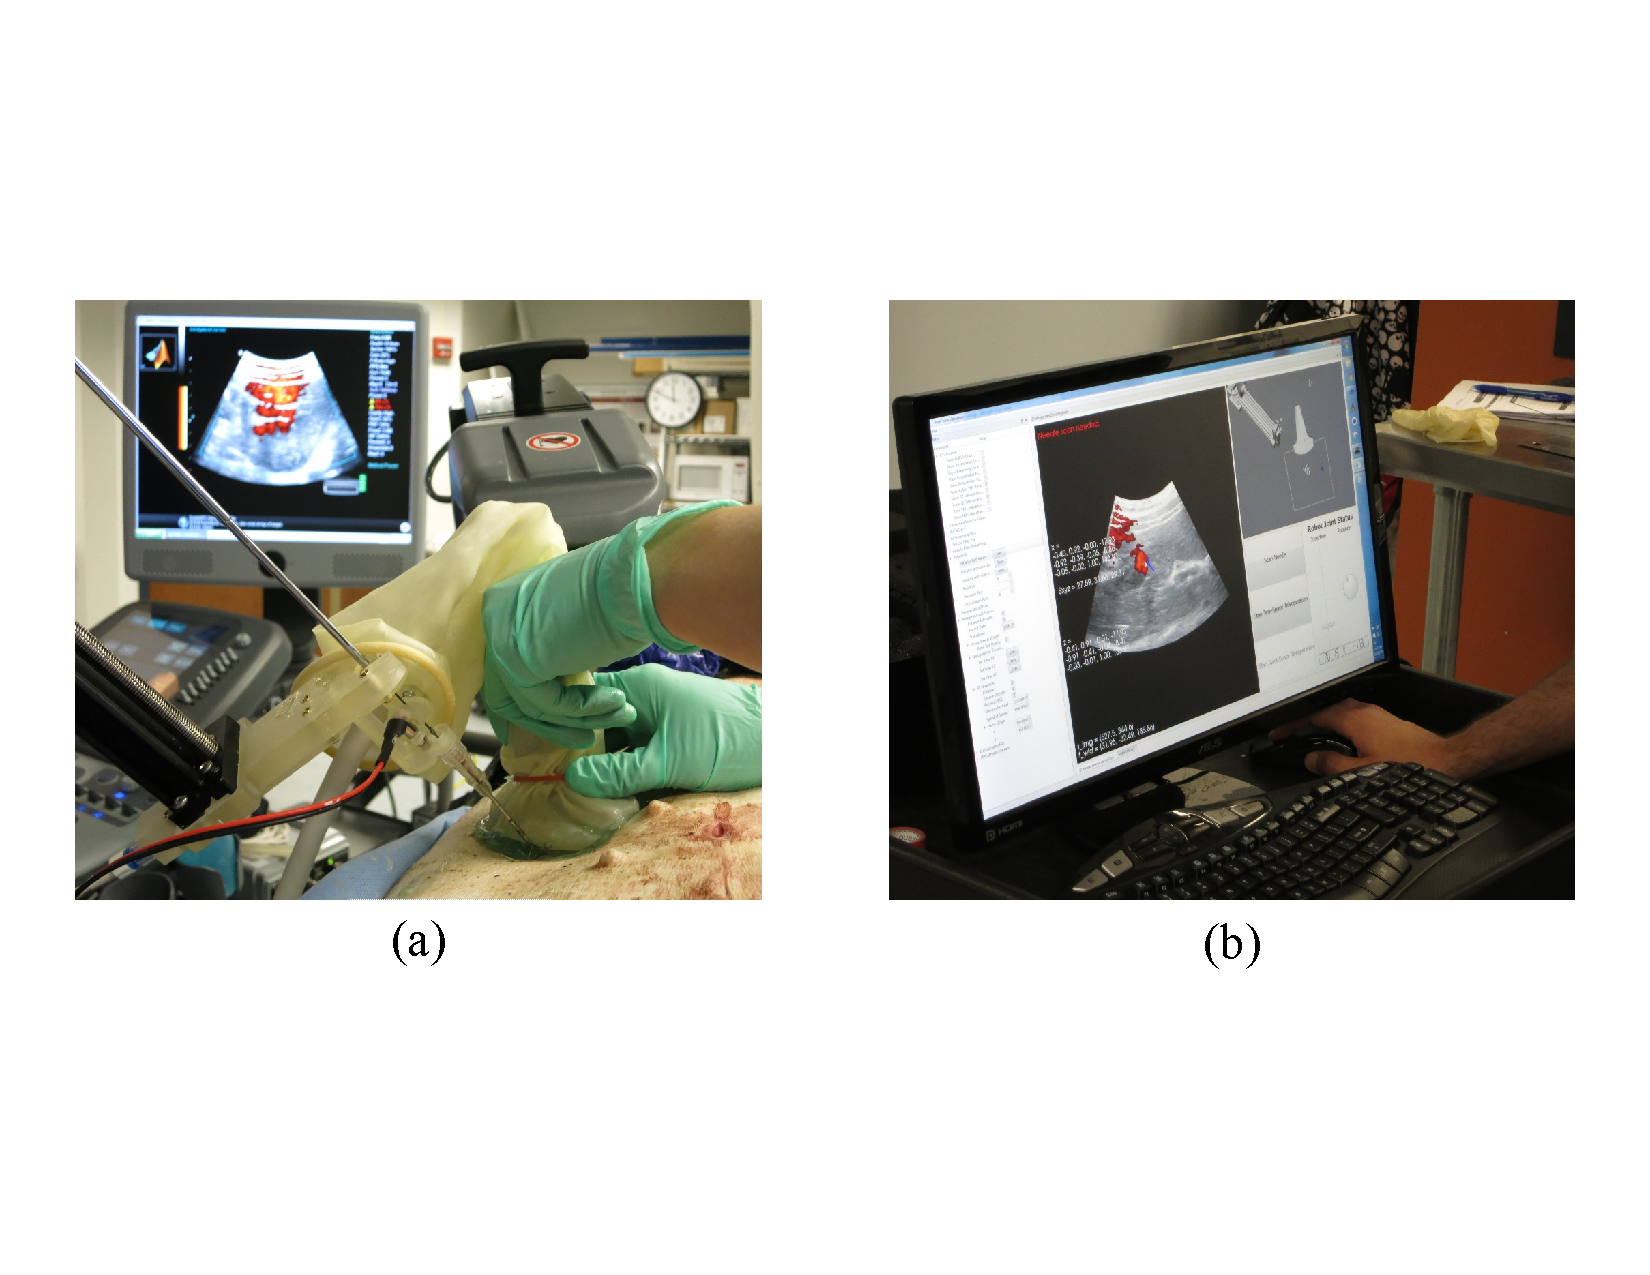
\includegraphics[width = \columnwidth]{./Images/Chapter5/CadaverUsers/CadaverUsers.pdf}%
\caption[User interactions during human-in-the-loop control]{User interactions during human-in-the-loop control: (a) One user manipulates the freehand-3D ultrasound transducer, scanning along the needle to localize the tip. (b) A second user interacts with the control software, selecting the location of the needle tip in an ultrasound image. }
\label{fig:CadaverUsers}
\end{figure} 

%------------------------------------------------------------------------------------------
%------------------------------------------------------------------------------------------
\section{Results and Discussion}
\label{sec:HumanInTheLoopResults}
%------------------------------------------------------------------------------------------
%------------------------------------------------------------------------------------------
\subsection{Quantification of Process and Measurement Noise}
Across 517 samples of process noise, the mean position error (in millimeters) and mean orientation error (in degrees) were \[{\overline{p}_{w}} = \begin{bmatrix} 0.03 &-0.17 &0.01 \end{bmatrix}^{\text{T}}, {\overline{r}_{w}} = \begin{bmatrix} 0.18 &-0.03 &0.08 \end{bmatrix}^{\text{T}}.\] To find the best-fit zero-mean Gaussian distribution to the process noise, we again reflected the measured noise vectors, resulting in a sample covariance of
\begin{align*}
{\hat{Q}} = \begin{bmatrix} 
\phantom{-}0.16 & \phantom{-}0.02 	&-0.04 & -0.01 & \phantom{-}0.03 & \phantom{-}0.06\\
\phantom{-}0.02 & \phantom{-}0.16 & -0.02 & -0.05 & \phantom{-}0.03 & \phantom{-}0.01 \\ 
-0.04 & -0.02 & \phantom{-}0.46 & -0.10 & \phantom{-}0.01 & -0.03 \\
-0.01 & -0.05 & -0.10 & \phantom{-}0.24 & \phantom{-}0.01 & \phantom{-}0.02 \\
\phantom{-}0.03 & \phantom{-}0.03 & \phantom{-}0.01 & \phantom{-}0.01 & \phantom{-}0.05 & \phantom{-}0.03 \\
\phantom{-}0.06 & -0.01 & -0.03 & \phantom{-}0.04 & \phantom{-}0.03 & \phantom{-}0.24\\ 
\end{bmatrix}.
\end{align*}

In the measurement noise experiment, we again assumed the mean of repeated localization at each tip pose was the true needle pose. Across 200 total measurements, the sample covariance was 
\begin{align*}
{\hat{R}} = \begin{bmatrix} 
\phantom{-}2.29 & \phantom{-}1.58 & \phantom{-}2.51 \\ 
\phantom{-}1.58 & \phantom{-}6.97 & \phantom{-}2.19 \\ 
\phantom{-}2.51 & \phantom{-}2.19 & \phantom{-}11.4 \\ 
\end{bmatrix}.
\end{align*}

\subsection{Accuracy of Estimation Scheme}
Across 5199 data points from four separate insertions, the mean distance between the estimator position estimate and the electromagnetic tracker measurement was 4.6~mm. Fig.~\ref{fig:UKFAccuracy} shows a comparison of the UKF estimator output and the electromagnetic tracking system, along with system inputs. Estimator error was generally largest in the robot frame's $y$-axis direction. In these tests, this corresponded to mismatches in the needle radius of curvature $\rho$. The UKF estimation scheme assumed a constant $\rho =$~85~mm once the steerable needle left the introducer needle. The value of $\rho = $~85~mm was based on initial measurements over complete insertions in the liver tissue sample. It should be noted that several practical issues limit the use of the electromagnetic tracker inside the needle tip as a gold standard. First, the tracker is sensitive to electromagnetic noise from the vibration motor during actual steering. Second, the vendor-supplied calibration of the tracked ultrasound transducer is not perfectly accurate. Finally, it is impossible to place the electromagnetic transducer right at the needle tip (because of the rigid bent-tip section), so a tip calibration must be applied to the raw tracking data. This tip calibration can become inaccurate as the needle bends, and makes the measurement very sensitive to orientation noise. 

\begin{figure}[!t]
\centering
\includegraphics[width = \columnwidth]{./Images/Chapter5/UKFAccuracy/UKFAccuracy.pdf}%
\caption[UKF accuracy results]{UKF estimation scheme accuracy results. Comparison of calibrated and filtered electromagnetic tracker position (GPS) with estimator position (UKF). Measurements are also indicated. Robot joint variables ($\theta$, $l$) and radius of curvature $\rho$ inputs to the model are also shown. For UKF updates, $\rho$ is set to 1000~mm while the needle is inside the introducer sheath. }
\label{fig:UKFAccuracy}
\end{figure}  

\subsection{Clinical Needle Steering Experiments}
Fig.~\ref{fig:CadaverDoppler} shows examples of in-plane and transverse power Doppler images of the vibrating needle in the cadaveric porcine liver. The disposable buzzer was able to generate a recognizable Doppler signature along the shaft of the needle in a realistic clinical imaging arrangement. The Doppler response tended to be more irregular and less localized during the initial insertion, especially while the steerable needle was still in the introducer needle. As seen in Fig.~\ref{fig:CadaverDoppler}(a), the image analysis methods presented in Chapter 2 would likely not have been able to generate a useful measurement of the tip pose. Once the steerable needle was inserted farther into the tissue, the Doppler response became more regular and localized around the steerable needle, as seen in Fig.~\ref{fig:CadaverDoppler}(b). 

\begin{figure}[!t]
\centering
\includegraphics[width = \columnwidth]{./Images/Chapter5/CadaverDoppler/CadaverDoppler.pdf}%
\caption[Power Doppler ultrasound images of steerable needle in pig cadaver]{Power Doppler ultrasound images of steerable needle in pig cadaver: (a) an in-plane image of the introducer needle and steerable needle. (b) A transverse image of the steerable needle.  }
\label{fig:CadaverDoppler}
\end{figure}  

Table~\ref{table:CadaverTargets} lists target positions, final joint variables, and tip placement error for the three targets. Target position $t$ is given relative to the starting position of the steerable needle based on the first measurement. For target 1, the final tip placement error measured in DynaCT was 4.24~mm, which approaches the level of accuracy needed in ablation of liver tumors. This target required less deviation from the initial insertion vector than target 2 and target 3. Fig.~\ref{fig:CadaverAtTarget} shows the software interface at the completion of steering to target 1. 


\begin{table}[!t]
% increase table row spacing, adjust to taste
\renewcommand{\arraystretch}{1.3}
\centering
\caption{Target positions and final error in clinical needle steering tests}
\label{table:CadaverTargets}
\begin{tabulary}{\columnwidth}{| C | C | C | C | C | C | C | }
\hline
Target & $t_x$ (mm) & $t_y$ (mm) & $t_z$ (mm) & $\theta_{\text{final}}$ (deg.) & $l_{\text{final}}$ (mm) & $e_{\text{final}} (mm)$ \\
\hline
1 & 8.9 & -2.3 & 72.3 & 233.2 & 71.7 & 4.24 \\
\hline
2 & 18.2 & -0.3 & 48.6 & -54.6 & 70.9 & 21.4 \\
\hline
2 & 49.5 & -35.1 & 61.7 & -128.3 & 140.1 & 21.4 \\
\hline
\end{tabulary}
\end{table}

For target 2, the intermediate target placed posterior to the gallbladder by puncturing the gallbladder sack, the final tip placement error measured in DynaCT was 24.24~mm. This target required a larger deviation from the initial insertion vector than target 1, and the final placement was correspondingly larger. The large final placement error appeared to be a result of poor curvature performance, rather than controller error. In other words, the estimation and control software kept the needle curving towards the target throughout insertion, the needle simply did not curve strongly enough to reach the target.

Target 3, the difficult target placed around the posterior aspect of the gallbladder, the final tip placement error measured in DynaCT was 24.24~mm. As with target 2, this again appeared to be a result of poor curvature performance.  

\begin{figure}[!t]
\centering
\includegraphics[width = \columnwidth]{./Images/Chapter5/CadaverAtTarget/CadaverAtTarget.jpg}%
\caption[Software interface at completion of clinical test]{Software interface at completion of clinical test with target 1. The estimator position (lines) is shown within the target icon (circle) in the live ultrasound image. A small Doppler response is seen at the needle tip. The target was located posterior to the gallbladder.}
\label{fig:CadaverAtTarget}
\end{figure}  

\subsection{Discussion}
Compared to bench-top testing using tissue specimens, steering in the cadaveric liver \textit{in situ} introduced several new factors that may have affected curvature performance. For example, connecting the needle steering robot to the introducer needle often required displacing the introducer needle relative to the surrounding tissue, which may have introduced a significant initial load on the needle as it exited the introducer inside the liver. Also, ultrasound imaging of the cadaveric liver involved much larger forces at the ultrasound transducer, resulting in displacement of the liver itself on the order of centimeters. 

Several important problems remain to be solved before our methods can be applied in a live-animal experiment. First, the mechanical behavior of bent-tip steerable needles in liver must be improved. Although our system was able to place the steerable needle tip at the three targets described in this chapter with varying levels of accuracy, in other anecdotal testing in the cadaveric liver, the needle tip frequently caught, occasionally causing severe buckling of the needle shaft. Although this was sometimes the result of impact with obvious anatomic structures such as fat or vasculature, as in earlier chapters, DynaCT images of the caught needle tip also occasionally showed no obvious impeding structure. In other words, the needle tip was not able to consistently cut through ordinary liver parenchyma. This mechanical catching might be greatly improved by producing steerable needles with sharper tips. In the current implementation the Nitinol flexure tip was sharpened using a grinding wheel, but the resulting edge was not nearly as sharp as a clinical trocar or introducer needle.

A second important problem is the management of respiratory motion. In the cadaver experiment described in this chapter, we elected not to ventilate the carcass to simulate respiratory motion. In a live-animal experiment, such motion is unavoidable. One strategy might be to gate control of the needle motion to the same portion of the respiratory cycle. Alternatively, high-frequency jet ventilation might be used to minimize respiratory motion.

A final important problem is the selection and placement of targets for the needle steering trials. It was remarkably difficult to place the introducer needle and fiducial markers to provide a realistic but feasible target geometry for each trial. Relative motion of the needles during connection of the robot, and displacement of the needles during penetration of the tough skin and subcutaneous fat were the main difficulties.


